\chapter{Servidor}

% Introdução ao programa servidor
%=====================================
No modelo cliente-servidor, o servidor é o elemento responsável por executar uma ação somente após um pedido realizado pelo cliente, sendo assim, o servidor deve estar sempre preparado para responder à uma solicitação de serviço. Deste modo, além da capacidade de se comunicar com o cliente, o servidor deve oferecer algum serviço de interesse do cliente. 

Neste trabalho o programa servidor disponibiliza ao cliente a interface com o FPGA presente no SoC, logo, ao receber o pedido do cliente, o servidor deve ser capaz de receber os dados vindos do cliente à unidade de processamento embarcada no FPGA e em seguida devolver esses dados já processados ao cliente. Entretanto, antes mesmo de iniciar o desenvolvimento do código do servidor, devemos compilar uma distribuição linux e configurar o processo de boot desse sistema no processador ARM presente no SoC. Estas etapas no desenvolvimento do servidor serão descritas neste capítulo.

% explicar processo de boot
%=====================================
\section{Processo de BOOT}
O fluxo de boot do linux na placa é resumido na Figura~\ref{fig:linux}. O primeiro elemento de software é o \textit{Boot ROM} que está gravado de fábrica internamente no dispositivo. Os arquivos de \textit{PreLoader},\textit{ U-boot} e do sistemas de aquivos do linux são salvos em um cartão de memória micro SD\@. O \textit{Secondary Program Loader - SPL}, conhecido como \textit{PreLoader}, é executado a partir da Boot ROM\@. Ele é responsável por configurar o sistema para que o \textit{bootloader} (U-boot) possa ser executado. A Intel fornece uma ferramenta chamada BSP editor que, a partir de arquivos que descrevem o hardware, podem gerar o PreLoader para o projeto específico~\cite{SocLinux}.  

\begin{figure}[ht]
	\caption{Boot linux embarcado}
	\begin{center}
		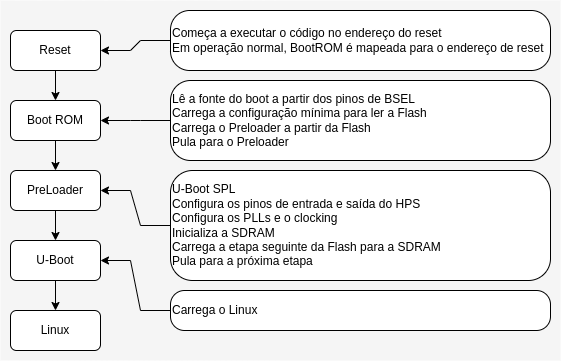
\includegraphics[scale=0.65]{imagens/embeddedLinux.png}\\
		{\small \textbf{Fonte:}\cite{SocLinux}}
    \end{center}\label{fig:linux}
\end{figure}

A etapa seguinte ao \textit{PreLoader} é o \textit{bootloader}. Nessa fase do boot todas as questões de baixo nível do SoC, como por exemplo, os clocks, pinos e SDRAM, já foram inicializados e estão prontos. O objetivo do bootloader, é obter essas informações do sistema e fazer com que ele funcione até o ponto onde o linux possa ser iniciado. Outra função importante do U-boot em um SoC Intel é programar o FPGA~\cite{SocLinux}.

% Explicar a distribuição usada
%=====================================
\section{Distribuição Linux rsyocto}
Com todos os arquivos necessários para o boot do sistema já gerados a partir das ferramentas de desenvolvimento da Intel, poderemos escolher nosso sistema operacional. O sistema escolhido foi uma distribuição linux desenvolvida exclusivamente para SoCs da Intel com fpga integrado, como pode ser observado na descrição da distribuição disponível em~\cite{rsyocto}:

\begin{citacao}
	``\textbf{rsyocto} is an open source Embedded Linux Distribution designed with the Yocto Project and with a custom build flow to be optimized for Intel SoC-FPGAs (Intel Cyclone V and Intel Arria 10 SX SoC-FPGA with an ARM Cortex-A9) to achieve the best customization for the strong requirements of modern embedded SoC-FPGA applications.''
\end{citacao} 

O rsyocto faz uso do Kernel Linux~\textbf{linux-socfpga 5.11}~\cite{linuxsocfpga} e possui um conjunto de ferramentas necessárias para ajudar a simplificar o uso e desenvolvimento de aplicações desenvolvidas para os SoCs com FPGA integrado da Intel. Além destas ferramentas o rsyocto dispõe de drivers para todos os periféricos de comunicação integrados SoC, como por exemplo, a interfaces I2C e CAN, e para todas as interfaces entres o HPS e o FPGA\@. O rsyocto oferece um conjunto de simples aplicações que podem ser executadas em linha de comando, que possibilitam executar novas configurações no FPGA, usando o FPGA Manager, até mesmo ler e escrever a interface ARM AXI-Bridge que permite interagir com o FPGA\@. 

Essas aplicações simplificam a comunicação com o FPGA a partir de simples comandos que podem ser executados a partir do terminal, através de todas as interfaces disponíveis, estes comandos são:~\textbf{lwhps2fpga}, que permite ações de leitura e escrita no barramento Lightweight HPS-to-FPGA-Bridge, o~\textbf{hps2fpga} para leitura e escrita no barramento HPS-to-FPGA-Bridge, o~\textbf{hps2sdram}, que proporciona acesso à interface da SDRAM e os~\textbf{gpi} e~\textbf{gpo} para acesso aos sinais de uso geral. Na Figura~\ref{fig:rsyocto} podemos ter uma visão geral de todas as ferramentas disponíveis na distribuição linux~\textit{rsyocto}.


\begin{figure}[ht]
	\caption{Overview do rsyocto}
	\begin{center}
		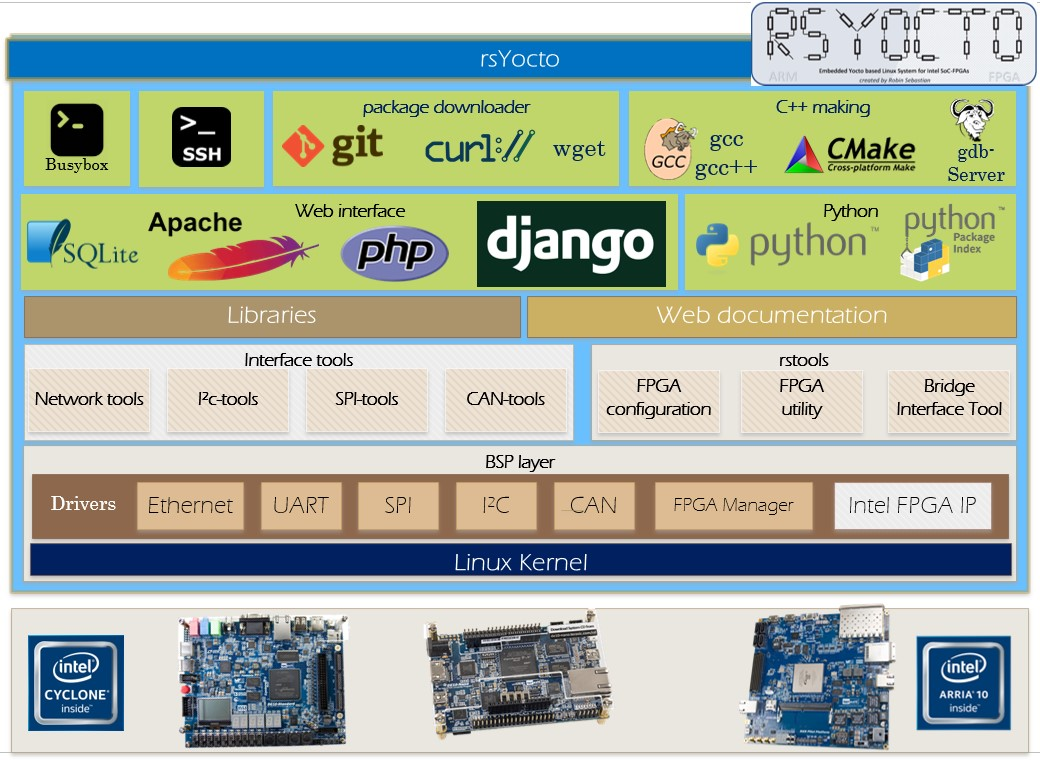
\includegraphics[scale=0.45]{imagens/rsYoctoLayers.jpg}\\
		{\small \textbf{Fonte:}\cite{rsyocto}}
    \end{center}\label{fig:rsyocto}
\end{figure}

A seguir são listadas algumas características da distribuição linux rsyocto que fazem dela uma excelente escolha para ser utilizada neste trabalho:
\begin{itemize}
	\item Embedded Linux specially developed for Intel SoC-FPGAs
	\item Linux Kernel 5.11 (Source)
	\item Full usage of the Dual-Core ARM (ARMv7-A) Cortex-A9 with
	\item FPGA Fabric configuration during the boot and with a single Linux command
	\item All Bridge Interfaces between the HPS and FPGA are enabled and ready for use!
	\item Tools to interact with the FPGA Fabric via the ARM AXI HPS-to-FPGA bridges
	\item HPS Hard IP components (I²C-,SPI-, CAN-BUS or UART) are routed to FPGA 
	\item USB Host support with test tools (e.g. lsusb)
	\item Full Linux Network stack with dynamic and static iPv4 is supported
	\item OpenSSH-Server starts automatically during boot
	\item gcccompiler 9.3.0; glibc and glib-2.0(The GNU C Library) cmake 3.16.5
	\item Python 3.8 Python3-dev and Python-dev
	\item git 2.31, wget 1.20.3, curl 7.69.1
	\item opkg package manager enables to add packages from different Linux Distributions.
	\item Changing the running FPGA-Configuration of the FPGA-Fabric
	\end{itemize}

% Explicar o códgo do servidor
%=====================================
\section{Interface socket server}
Com o linux já devidamente configurado, ele já pode ser inicializado no processador do SoC, assim podemos iniciar o desenvolvimento do servidor. No primeiro momento devemos realizar o download do código fonte da biblioteca de comunicação, a libinterfacesocket, que já foi detalhada anteriormente, o código fonte pode ser baixado em~\cite{interface-socket-server}. Com os arquivos já no sistema de diretórios do SoC devemos realizar a compilação e a instalação da libinterfacesocket, só assim o servidor terá acesso a suas funcionalidades. 

Logo que é inicializado o servidor mantém uma porta aberta para estabelecer uma conexão com o cliente e assim que a conexão é estabelecida, o cliente já pode começar a enviar os dados. Ao receber os dados do cliente, o servidor envia-os ao FPGA que os processa e os devolve ao servidor para que ele possa reenviar os dados já processados ao cliente. Um fluxograma simplificado desse processo pode ser visualizado na Figura \ref{fig:fluxoServidor}.

\begin{figure}[ht]
	\caption{Fluxograma simplificado do servidor}
	\begin{center}
		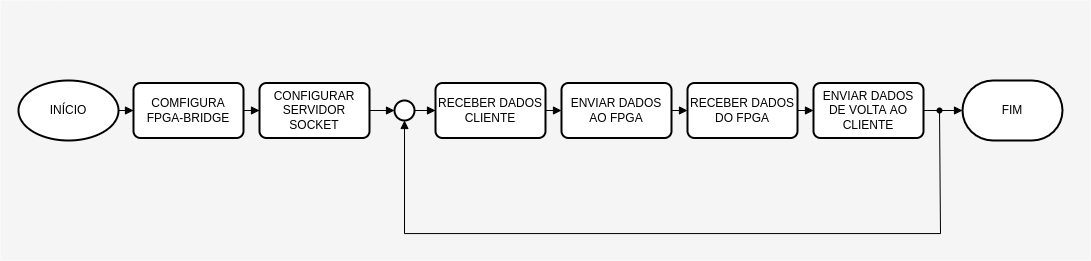
\includegraphics[scale=0.41]{imagens/fluxogramaServidor.png}\\
		{\small \textbf{Fonte:}Elaborado pelo autor}
    \end{center}\label{fig:fluxoServidor}
\end{figure} 

O acesso do servidor ao FPGA é feito através de mapeamento de endereços do linux, os SoCs Intel possuem uma arquitetura de memória mapeada. Desta forma, além da biblioteca desenvolvida durante a pesquisa, um outro arquivo cabeçalho é necessário para facilitar o acesso aos endereços de memória do HPS\@. Quando uma instância do processador ARM é incluída no projeto do QSys Designer, é gerado um arquivo.sopcinfo no momento em que o projeto é compilado. Podemos usar esse arquivo como entrada da ferramenta \textit{sopc-create-header-files} presente no SoC EDS para gerar um novo arquivo com extensão \textit{.h}, que lista os endereços base de todos os módulos (IP) incluídos no FPGA\@. 

Portanto, o arquivo cabeçalho gerado disponibiliza o \textit{offset} do endereço em que cada periférico está localizado para cada uma das FPGA-bridges disponíveis. Deste modo o servidor pode enviar ou receber dados ao periférico conhecendo o endereço da FPGA-bridge em que este periférico está conectado e o seu nome, sem a necessidade de se conhecer exatamente o seu endereço. Na Figura~\ref{fig:codigodobro} é apresentado uma parte do arquivo cabeçalho gerado pela ferramenta sopc-create-reader-files, neste trecho são realizadas algumas definições que facilitam o acesso ao IP dobro, que já está instanciado no FPGA\@. Este módulo IP foi usado para testar o processo completo de comunicação entre o tópico ROS até o FPGA\@.

\begin{figure}[ht]
\caption{Definição de endereço presente no arquivo hps\underline{ }0.h}
\begin{center}
\begin{lstlisting}[language=C++, backgroundcolor=\color{gray!10}]
 /*
 * Macros for device 'Dobro_0', class 'Dobro'
 * The macros are prefixed with 'DOBRO_0_'.
 * The prefix is the slave descriptor.
 */
 #define DOBRO_0_COMPONENT_TYPE Dobro
 #define DOBRO_0_COMPONENT_NAME Dobro_0
 #define DOBRO_0_BASE 0x38
 #define DOBRO_0_SPAN 4
 #define DOBRO_0_END 0x3b
\end{lstlisting}
{\small \textbf{Fonte:}Elaborado pelo autor}	
\end{center}\label{fig:codigodobro}
\end{figure}


Para interagir com FPGA usando o recurso de memória mapeada, a primeira coisa que devemos fazer é abrir o dispositivo de memória do sistema. Em distribuições linux o acesso à memória física do sistema é realizado através do dispositivo /dev/mem, esse dispositivo funciona como um arquivo caracteres que representa uma imagem da memória principal do computador~\cite{manmem}. Por se comportar como um arquivo no sistema, podemos no programa abri-lo como abriríamos qualquer arquivo de caracteres, com a funções \textit{open}, como pode ser visto na linha 2 da Figura~\ref{fig:codigomap}.

Em seguida podemos usar o descritor de arquivo gerado como retorno da função open, para criar um ponteiro, que dará acesso à memória principal do sistema. Para gerarmos este ponteiro, podemos usar a função mmap, ela cria um mapeamento virtual no espaço de endereço passado como argumento da função. Nos dois primeiros argumentos da função mmap, como pode ser visto na linha 10 da Figura~\ref{fig:codigomap},  podemos definir o espaço de endereços para o mapeamento. No código apresentado este espaço se inicial no endereço zero, NULL\@, e termina na constante HPS\underline{ }TO\underline{ }FPGA\underline{ }AXI\underline{ }SPAN (0x3C000000), que guarda o valor do alcance máximo do espaço de endereço das interfaces entre o HPS e o FPGA\@. O ultimo argumento da função mmap é o endereço base da Lightweight HPS-to-FPGA-Bridge (0xC0000000), representado pela constante HPS\underline{ }TO\underline{ }FPGA\underline{ }AXI\underline{ }BASE.



\begin{figure}[ht]
\caption{Memória mapeada}
\begin{center}
\begin{lstlisting}[language=C++, backgroundcolor=\color{gray!10}]
 // Open up the /dev/mem device
 devmem_fd = open("/dev/mem", O_RDWR | O_SYNC);
 if(devmem_fd < 0) {
	perror("devmem open"); 
	exit(EXIT_FAILURE);
 }	

 // mmap() the entire address space of the Lightweight 
 // bridge so we can access our custom module 
 lw_bridge_map = (uint32_t *)mmap( 
				NULL, 
				HPS_TO_FPGA_AXI_SPAN, 
				PROT_READ|PROT_WRITE, 
				MAP_SHARED, 
				devmem_fd, 
				HPS_TO_FPGA_AXI_BASE ); 
				
 if(lw_bridge_map == MAP_FAILED) {
	perror("devmem mmap");
	close(devmem_fd);
	exit(EXIT_FAILURE);
 }
\end{lstlisting}
{\small \textbf{Fonte:}Elaborado pelo autor}	
\end{center}\label{fig:codigomap}
\end{figure} 

Agora que já existe um ponteiro para a região de memória onde se encontra a interface de comunicação com o FPGA, podemos enviar e receber dados para o IP instanciado no FPGA. Para isto, vamos usar este ponteiro para o endereço da HPS-to-FPGA-Bridge, somado com o offset presente no arquivo hps\underline{ }0.h.  Consequentemente, será possível interagir com o IP em um programa escrito em linguagem C, da mesma maneira que interagimos com um ponteiro comum. O bloco de código da Figura~\ref{fig:codigomapdobro} ilustra este processo de escrita e leitura de dados em um IP através de um ponteiro

\begin{figure}[ht]
\caption{Memória mapeada}
\begin{center}
\begin{lstlisting}[language=C++, backgroundcolor=\color{gray!10}]
 // Set the dobro_map to the correct offset within the RAM
 uint32_t * dobro_map = 0;
 dobro_map = (uint32_t*)(lw_bridge_map + DOBRO_0_BASE);

 *dobro_map = 56;
 valor = *dobro_map;
\end{lstlisting}
{\small \textbf{Fonte:}Elaborado pelo autor}	
\end{center}\label{fig:codigomapdobro}
	
\end{figure}